\documentclass{standalone}
\usepackage{tikz}
\usetikzlibrary{patterns, positioning}

\begin{document}
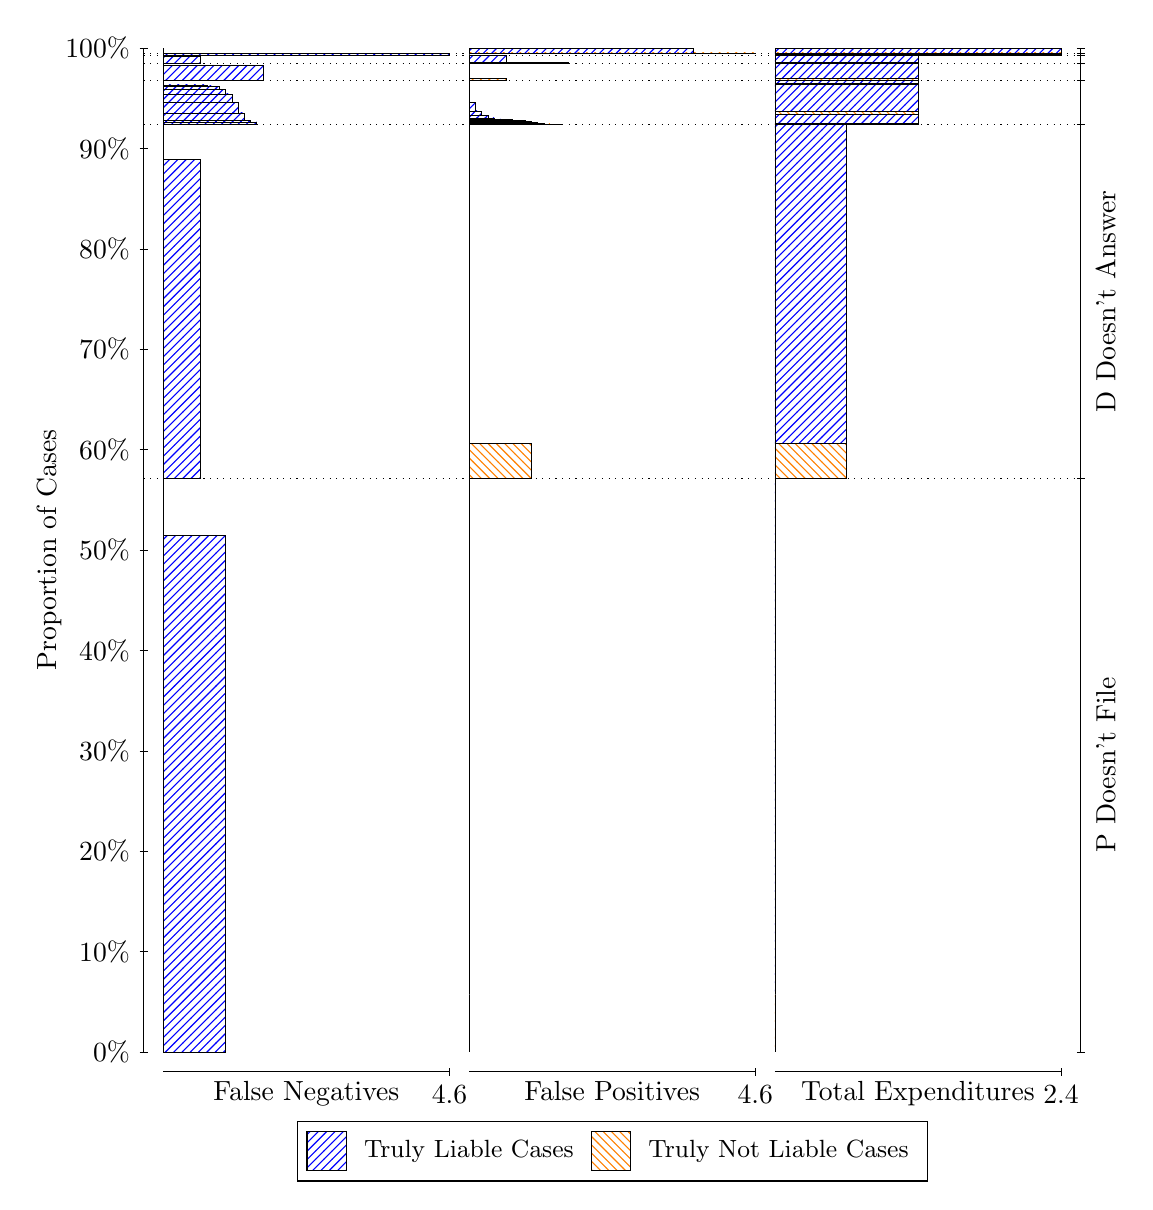
\begin{tikzpicture}
\draw[black, very thin] (1.5,1.75) -- (1.5,14.5);
\node[rotate=90, anchor=center] at (0.3, 8.125) {Proportion of Cases};
\draw[black, very thin] (1.45,1.75) -- (1.55,1.75);
\node[anchor=east] at (1.45, 1.75) {0\%};
\draw[black, very thin] (1.45,3.025) -- (1.55,3.025);
\node[anchor=east] at (1.45, 3.025) {10\%};
\draw[black, very thin] (1.45,4.3) -- (1.55,4.3);
\node[anchor=east] at (1.45, 4.3) {20\%};
\draw[black, very thin] (1.45,5.575) -- (1.55,5.575);
\node[anchor=east] at (1.45, 5.575) {30\%};
\draw[black, very thin] (1.45,6.85) -- (1.55,6.85);
\node[anchor=east] at (1.45, 6.85) {40\%};
\draw[black, very thin] (1.45,8.125) -- (1.55,8.125);
\node[anchor=east] at (1.45, 8.125) {50\%};
\draw[black, very thin] (1.45,9.4) -- (1.55,9.4);
\node[anchor=east] at (1.45, 9.4) {60\%};
\draw[black, very thin] (1.45,10.675) -- (1.55,10.675);
\node[anchor=east] at (1.45, 10.675) {70\%};
\draw[black, very thin] (1.45,11.95) -- (1.55,11.95);
\node[anchor=east] at (1.45, 11.95) {80\%};
\draw[black, very thin] (1.45,13.225) -- (1.55,13.225);
\node[anchor=east] at (1.45, 13.225) {90\%};
\draw[black, very thin] (1.45,14.5) -- (1.55,14.5);
\node[anchor=east] at (1.45, 14.5) {100\%};

\draw[black, very thin] (13.4,1.75) -- (13.4,14.5);
\draw[black, very thin] (13.35,1.75) -- (13.45,1.75);
\node[anchor=west] at (13.35, 1.75) {};
\draw[black, very thin] (13.35,9.0384) -- (13.45,9.0384);
\node[anchor=west] at (13.35, 9.0384) {};
\draw[black, very thin] (13.35,13.532) -- (13.45,13.532);
\node[anchor=west] at (13.35, 13.532) {};
\draw[black, very thin] (13.35,14.088) -- (13.45,14.088);
\node[anchor=west] at (13.35, 14.088) {};
\draw[black, very thin] (13.35,14.304) -- (13.45,14.304);
\node[anchor=west] at (13.35, 14.304) {};
\draw[black, very thin] (13.35,14.409) -- (13.45,14.409);
\node[anchor=west] at (13.35, 14.409) {};
\draw[black, very thin] (13.35,14.435) -- (13.45,14.435);
\node[anchor=west] at (13.35, 14.435) {};
\draw[black, very thin] (13.35,14.5) -- (13.45,14.5);
\node[anchor=west] at (13.35, 14.5) {};

\draw[black, very thin, pattern color=blue, pattern=north east lines] (1.75,1.75) rectangle (2.5399,8.3096);
\draw[black, very thin, pattern color=orange, pattern=north west lines] (1.75,8.3096) rectangle (1.75,9.0384);
\draw[black, very thin, pattern color=blue, pattern=north east lines] (1.75,9.0384) rectangle (2.2239,13.087);
\draw[black, very thin, pattern color=orange, pattern=north west lines] (1.75,13.087) rectangle (1.75,13.532);
\draw[black, very thin, pattern color=blue, pattern=north east lines] (1.75,13.532) rectangle (2.9348,13.561);
\draw[black, very thin, pattern color=blue, pattern=north east lines] (1.75,13.561) rectangle (2.8558,13.579);
\draw[black, very thin, pattern color=blue, pattern=north east lines] (1.75,13.579) rectangle (2.7768,13.676);
\draw[black, very thin, pattern color=blue, pattern=north east lines] (1.75,13.676) rectangle (2.6978,13.808);
\draw[black, very thin, pattern color=blue, pattern=north east lines] (1.75,13.808) rectangle (2.6188,13.918);
\draw[black, very thin, pattern color=blue, pattern=north east lines] (1.75,13.918) rectangle (2.5399,13.977);
\draw[black, very thin, pattern color=blue, pattern=north east lines] (1.75,13.977) rectangle (2.4609,14.008);
\draw[black, very thin, pattern color=blue, pattern=north east lines] (1.75,14.008) rectangle (2.3819,14.02);
\draw[black, very thin, pattern color=blue, pattern=north east lines] (1.75,14.02) rectangle (2.3029,14.031);
\draw[black, very thin, pattern color=orange, pattern=north west lines] (1.75,14.031) rectangle (1.75,14.088);
\draw[black, very thin, pattern color=blue, pattern=north east lines] (1.75,14.088) rectangle (3.0138,14.28);
\draw[black, very thin, pattern color=orange, pattern=north west lines] (1.75,14.28) rectangle (1.75,14.304);
\draw[black, very thin, pattern color=blue, pattern=north east lines] (1.75,14.304) rectangle (2.2239,14.399);
\draw[black, very thin, pattern color=orange, pattern=north west lines] (1.75,14.399) rectangle (1.75,14.409);
\draw[black, very thin, pattern color=blue, pattern=north east lines] (1.75,14.409) rectangle (5.3833,14.427);
\draw[black, very thin, pattern color=orange, pattern=north west lines] (1.75,14.427) rectangle (1.75,14.435);
\draw[black, very thin, pattern color=orange, pattern=north west lines] (1.75,14.435) rectangle (1.75,14.437);
\draw[black, very thin, pattern color=blue, pattern=north east lines] (1.75,14.437) rectangle (1.75,14.5);
\draw[black, very thin, pattern color=orange, pattern=north west lines] (5.6333,1.75) rectangle (5.6333,2.4788);
\draw[black, very thin, pattern color=blue, pattern=north east lines] (5.6333,2.4788) rectangle (5.6333,9.0384);
\draw[black, very thin, pattern color=orange, pattern=north west lines] (5.6333,9.0384) rectangle (6.4232,9.4829);
\draw[black, very thin, pattern color=blue, pattern=north east lines] (5.6333,9.4829) rectangle (5.6333,13.532);
\draw[black, very thin, pattern color=orange, pattern=north west lines] (5.6333,13.532) rectangle (6.8181,13.533);
\draw[black, very thin, pattern color=orange, pattern=north west lines] (5.6333,13.533) rectangle (6.7391,13.535);
\draw[black, very thin, pattern color=orange, pattern=north west lines] (5.6333,13.535) rectangle (6.6601,13.538);
\draw[black, very thin, pattern color=orange, pattern=north west lines] (5.6333,13.538) rectangle (6.5812,13.545);
\draw[black, very thin, pattern color=orange, pattern=north west lines] (5.6333,13.545) rectangle (6.5022,13.558);
\draw[black, very thin, pattern color=orange, pattern=north west lines] (5.6333,13.558) rectangle (6.4232,13.572);
\draw[black, very thin, pattern color=orange, pattern=north west lines] (5.6333,13.572) rectangle (6.3442,13.583);
\draw[black, very thin, pattern color=orange, pattern=north west lines] (5.6333,13.583) rectangle (6.2652,13.585);
\draw[black, very thin, pattern color=orange, pattern=north west lines] (5.6333,13.585) rectangle (6.1862,13.589);
\draw[black, very thin, pattern color=blue, pattern=north east lines] (5.6333,13.589) rectangle (6.0283,13.6);
\draw[black, very thin, pattern color=blue, pattern=north east lines] (5.6333,13.6) rectangle (5.9493,13.612);
\draw[black, very thin, pattern color=blue, pattern=north east lines] (5.6333,13.612) rectangle (5.8703,13.643);
\draw[black, very thin, pattern color=blue, pattern=north east lines] (5.6333,13.643) rectangle (5.7913,13.702);
\draw[black, very thin, pattern color=blue, pattern=north east lines] (5.6333,13.702) rectangle (5.7123,13.812);
\draw[black, very thin, pattern color=blue, pattern=north east lines] (5.6333,13.812) rectangle (5.6333,14.088);
\draw[black, very thin, pattern color=orange, pattern=north west lines] (5.6333,14.088) rectangle (6.1072,14.113);
\draw[black, very thin, pattern color=blue, pattern=north east lines] (5.6333,14.113) rectangle (5.6333,14.304);
\draw[black, very thin, pattern color=orange, pattern=north west lines] (5.6333,14.304) rectangle (6.8971,14.314);
\draw[black, very thin, pattern color=blue, pattern=north east lines] (5.6333,14.314) rectangle (6.1072,14.409);
\draw[black, very thin, pattern color=orange, pattern=north west lines] (5.6333,14.409) rectangle (5.6333,14.417);
\draw[black, very thin, pattern color=blue, pattern=north east lines] (5.6333,14.417) rectangle (5.6333,14.435);
\draw[black, very thin, pattern color=orange, pattern=north west lines] (5.6333,14.435) rectangle (9.2667,14.437);
\draw[black, very thin, pattern color=blue, pattern=north east lines] (5.6333,14.437) rectangle (8.4768,14.5);
\draw[black, very thin, pattern color=orange, pattern=north west lines] (9.5167,1.75) rectangle (9.5167,2.4788);
\draw[black, very thin, pattern color=blue, pattern=north east lines] (9.5167,2.4788) rectangle (9.5167,9.0384);
\draw[black, very thin, pattern color=orange, pattern=north west lines] (9.5167,9.0384) rectangle (10.425,9.4829);
\draw[black, very thin, pattern color=blue, pattern=north east lines] (9.5167,9.4829) rectangle (10.425,13.532);
\draw[black, very thin, pattern color=orange, pattern=north west lines] (9.5167,13.532) rectangle (11.333,13.544);
\draw[black, very thin, pattern color=blue, pattern=north east lines] (9.5167,13.544) rectangle (11.333,13.654);
\draw[black, very thin, pattern color=orange, pattern=north west lines] (9.5167,13.654) rectangle (11.333,13.693);
\draw[black, very thin, pattern color=blue, pattern=north east lines] (9.5167,13.693) rectangle (11.333,14.041);
\draw[black, very thin, pattern color=orange, pattern=north west lines] (9.5167,14.041) rectangle (11.333,14.046);
\draw[black, very thin, pattern color=blue, pattern=north east lines] (9.5167,14.046) rectangle (11.333,14.088);
\draw[black, very thin, pattern color=orange, pattern=north west lines] (9.5167,14.088) rectangle (11.333,14.113);
\draw[black, very thin, pattern color=blue, pattern=north east lines] (9.5167,14.113) rectangle (11.333,14.304);
\draw[black, very thin, pattern color=orange, pattern=north west lines] (9.5167,14.304) rectangle (11.333,14.314);
\draw[black, very thin, pattern color=blue, pattern=north east lines] (9.5167,14.314) rectangle (11.333,14.409);
\draw[black, very thin, pattern color=orange, pattern=north west lines] (9.5167,14.409) rectangle (13.15,14.417);
\draw[black, very thin, pattern color=blue, pattern=north east lines] (9.5167,14.417) rectangle (13.15,14.435);
\draw[black, very thin, pattern color=orange, pattern=north west lines] (9.5167,14.435) rectangle (13.15,14.437);
\draw[black, very thin, pattern color=blue, pattern=north east lines] (9.5167,14.437) rectangle (13.15,14.5);
\draw[black, dotted] (1.5,9.0384) -- (13.4,9.0384);
\draw[black, dotted] (1.5,13.532) -- (13.4,13.532);
\draw[black, dotted] (1.5,14.088) -- (13.4,14.088);
\draw[black, dotted] (1.5,14.304) -- (13.4,14.304);
\draw[black, dotted] (1.5,14.409) -- (13.4,14.409);
\draw[black, dotted] (1.5,14.435) -- (13.4,14.435);
\draw[black, very thin] (1.75,1.5) -- (5.3833,1.5);
\node[anchor=north] at (3.5667, 1.5) {False Negatives};
\draw[black, very thin] (5.3833,1.45) -- (5.3833,1.55);
\node[anchor=north] at (5.3833, 1.45) {4.6};

\draw[black, very thin] (5.6333,1.5) -- (9.2667,1.5);
\node[anchor=north] at (7.45, 1.5) {False Positives};
\draw[black, very thin] (9.2667,1.45) -- (9.2667,1.55);
\node[anchor=north] at (9.2667, 1.45) {4.6};

\draw[black, very thin] (9.5167,1.5) -- (13.15,1.5);
\node[anchor=north] at (11.333, 1.5) {Total Expenditures};
\draw[black, very thin] (13.15,1.45) -- (13.15,1.55);
\node[anchor=north] at (13.15, 1.45) {2.4};

\node[black, centered, rotate=90] at (13.72, 5.3942) {P Doesn't File};
\node[black, centered, rotate=90] at (13.72, 11.285) {D Doesn't Answer};






\draw (7.449999999999999,1.5) node[draw=none] (baseCoordinate) {};
\begin{scope}[align=center]
        \matrix[scale=0.5, draw=black, below=0.5cm of baseCoordinate, nodes={draw}, column sep=0.1cm]{
            \node[rectangle, draw, minimum width=0.5cm, minimum height=0.5cm, pattern=north east lines, pattern color=blue] {}; &
            \node[draw=none, font=\small] (B) {Truly Liable Cases}; &
            \node[rectangle, draw, minimum width=0.5cm, minimum height=0.5cm, pattern=north west lines, pattern color=orange] {}; &
            \node[draw=none, font=\small] (B) {Truly Not Liable Cases}; \\
            };
\end{scope}

\end{tikzpicture}
\end{document}